\newpage
\section{Incorporating Sparsity into Scaling Laws}
\label{appendix:scaling_law_sparsity}

\Cref{tab:lbfgs:hparams} shows the parameters used to initialize L-BFGS used to fit the proposed parametric scaling law given in~\Cref{eq:loss:moe:proposal1}. \Cref{tab:lbfgs:estimate_params} shows the estimated parameters for the parameteric model. We use a held out dataset that consists of data points for models with sparsity value $S = 0.98$ to validate the performance of the estimated model coefficients. The mean squared error and the Huber loss error on the dataset used to fit the model is $0.00056$ and $ 0.0036$ respectively and $0.0058$ and $0.0011$ respectively on the out-of-sample validation set. The quality of the fit measured via the $R^{2}$ metric is $99\%$ on fitting data and $68\%$ on the held out validation dataset.

% \begin{table*}[h]
%     % VT notebook to equation mapping
%     % a, \alpha is C, \lambda
%     \centering
%     \caption{Initial values used to estimate coefficients in \Cref{eq:loss:moe:proposal1}.}
%     \begin{tabular}{c c c c}
%     \toprule
%     $\log(a)$, $\log(b)$, $\log(c)$, $\log(d)$ & $\alpha$, $\beta$, $\gamma$ & $\lambda$, $\delta$ & $\log(e)$ \\
%     \midrule
%     $\left[0, 10, 20 \right]$ & $\left[ 0, 0.25, 0.5, 0.75, 1, 1.25\right]$ & $\left[ -1, -0.5, 0, 0.5, 1\right]$ & $1.5$ \\
%     \bottomrule
%     \end{tabular}
% \label{tab:lbfgs:hparams}
% \end{table*}

% \begin{figure}[ht]
%     \centering
%     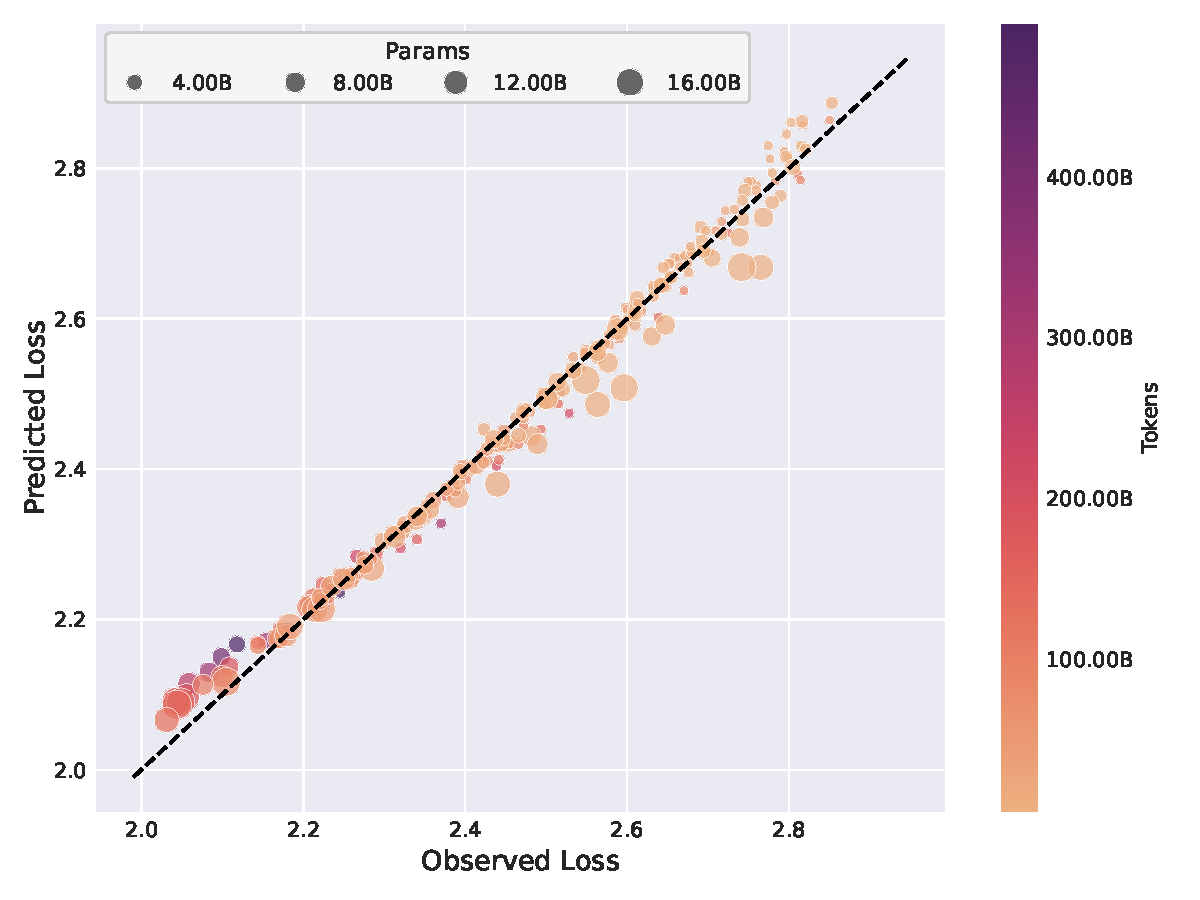
\includegraphics[width=0.48\textwidth]{plots/parameteric_law_interpolation.pdf}
%     \caption{Scaling law fit on data used to estimate coefficients for~\Cref{eq:loss:moe:proposal1}. All $S = 0.98$ data points are excluded from the fitting process to provide an out-of-sample validation show in~\Cref{fig:scaling_law:sparsity98}}.
%     \label{fig:scaling_law:in_sample}
% \end{figure}

\begin{table*}[h]
    % VT notebook to equation mapping
    % a, \alpha is C, \lambda
    \centering
    \caption{Initial values used to estimate coefficients in \Cref{eq:loss:moe:proposal1}.}
    \begin{tabular}{c | c}
    \toprule
    Coefficients & Initial Values \\
    \midrule
    $\log(a)$, $\log(b)$, $\log(c)$, $\log(d)$ & $\left[0, 10, 20 \right]$ \\
    $\alpha$, $\beta$, $\gamma$ & $\left[ 0, 0.25, 0.5, 0.75, 1, 1.25\right]$ \\ 
    $\lambda$, $\delta$ & $\left[ -1, -0.5, 0, 0.5, 1\right]$\\
    $\log(e)$ & $1.5$  \\
    \bottomrule
    \end{tabular}
\label{tab:lbfgs:hparams}
\end{table*}

\begin{table*}[h]
    % VT notebook to equation mapping
    % a, \alpha is C, \lambda
    \centering
    \caption{Estimated values for coefficients in \Cref{eq:loss:moe:proposal1}.}
    \begin{tabular}{c | c}
    \toprule
    Coefficient & Estimate \\
    \midrule
    $\alpha$ & 0.5962 \\
    $\beta$ & 0.3954 \\
    $\lambda$ & -0.1666 \\
    $\delta$ & 0.1603\\
    $\gamma$ & 0.1595 \\
    a & 16612.50 \\
    b & 5455.67 \\
    c & 0.4598 \\
    d & 17.26 \\
    e & 0.94 \\    
    \bottomrule
    \end{tabular}
\label{tab:lbfgs:estimate_params}
\end{table*}